\documentclass[]{scrartcl}

\usepackage {listings}
\usepackage[ngerman]{babel}
\usepackage[utf8]{inputenc}
\usepackage{graphicx}
\usepackage{xcolor}
\usepackage{hyperref}

\setlength{\parindent}{0em}


%opening
\title{Warenlagerung eines Kaufhauses}
\subtitle{Evolutionäre Algorithmen - SL3 - Soft Computing - SS17}
\author{Benedikt Straube}

\begin{document}

\maketitle

\newpage

\section{Installation}
Zur lokalen Ausführung der Applikation ist eine NodeJs Installation notwendig. Diese sollte mindestens in Version 6.11.0 (\url{https://nodejs.org/}) zur Verfügung stehen.

Im nächsten Schritt sollten innerhalb des Projektverzeichnisses die notwendigen Pakete für eine lokale Ausführung installiert werden. Dies ist möglich via 
\begin{lstlisting}[backgroundcolor=\color{lightgray}]
npm install
\end{lstlisting}

Nachdem alle notwendigen Pakete installiert wurden, kann ein lokaler Server mittels
\begin{lstlisting}[backgroundcolor=\color{lightgray}]
npm start
\end{lstlisting}
gestartet werden.

Danach ist die Applikation im Browser über \url{http:localhost:4200} zu erreichen.

\newpage
\section{Ausführung}
\label{ausfuehrung}
Die Applikation kann über die beschriebe Installation lokal gestartet und über den Browser bedient werden. Weiterhin wird der compilierte Code zusätzlich über GitHub-Pages gehostet. Dadurch ist die Applikation auch unter der URL \url{https://benediktst.github.io/Soft-Computing-VAWI} zu erreichen.

Vorsicht: Hier existiert zum aktuellen Zeitpunkt noch ein Bug des Routings, was bei dem Refresh der Applikation zu einer 404-Seite führt. Die Applikation kann immer wieder über die Angegebene URL erreicht werden.

\begin{figure}[htbp]
	\centering
	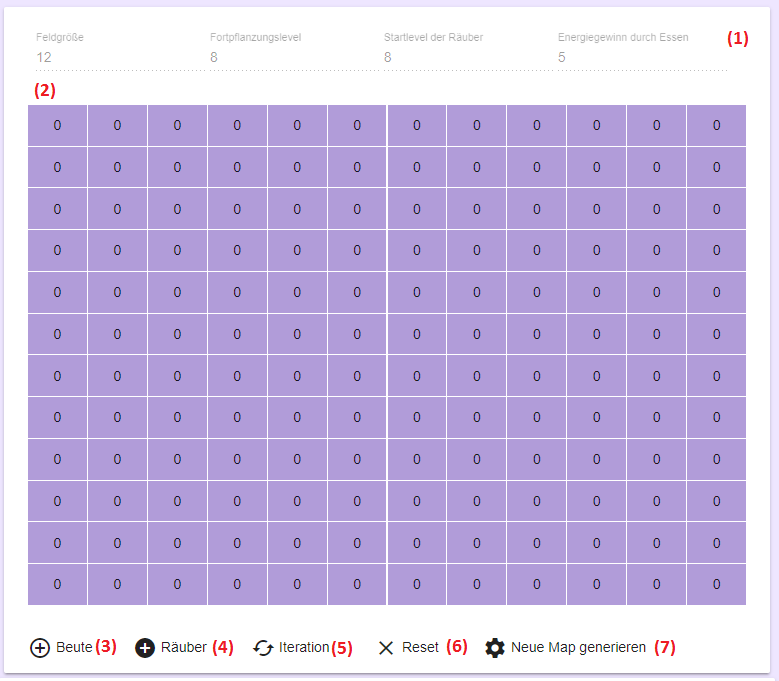
\includegraphics[width=0.8\textwidth]{res/interface.png}
	\caption{Aktionsmöglichkeiten der Anwendung}
	\label{img:interface}
\end{figure}

Um die Implementierung der SL-3 zu erreichen muss innerhalb der Kopfzeile ganz rechts das Menü geöffnet und die Option SL-3 ausgewählt werden. In der Anwendung (siehe Abbildung \ref{img:interface}) können an erster Stelle (1) die Ausgangsdaten eingesehen werden. Diese sind für diese Implementierung statisch im Code hinterlegt und sind hier lediglich informativ. Bei den Aktionen steht zuerst die Generierung der Kinder (2) zur Verfügung. Dies geschieht nach einer Evolutionsstrategie (ES), welche in Abschnitt \ref{logik} genauer erläutert wird. Die Bewertung (3) fügt eine Bewertung zu jedem Vektor hinzu. Die Eltern erhalten ebenfalls eine Bewertung, auch wenn sie für nie nachfolgende Generation nicht weiter betrachtet werden. Bei der Mutation (4) wird eine statische Standardabweichung auf alle Bestandteile der Vektoren angewendet, um die notwendige Varianz zu erhalten. Die dadurch entstehenden Vektoren werden dann als neue Elterngeneration verwendet. Bei der 50-fachen Iteration (5) werden die vorherigen drei Schritte entsprechend häufig wiederholt. Per (6) kann die Konfiguration der ES angepasst werden, was nachfolgend noch genauer dargestellt wird. Durch (7) wird der Ausgangszustand wieder hergestellt.\\

\begin{figure}[htbp]
	\centering
	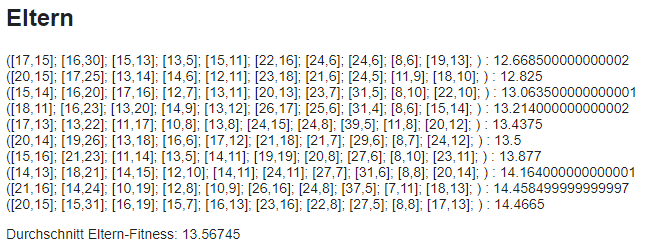
\includegraphics[width=0.8\textwidth]{res/vektoren.png}
	\caption{Darstellung der Vektoren}
	\label{img:vektoren}
\end{figure}

Abbildung \ref{img:vektoren} zeigt die Darstellung der Vektoren. Unter (1) werden die Vektoren der Elterngeneration angezeigt. Zusätzlich ist unter (2) die durchschnittliche Fitness der Eltern dargestellt und unter (3) der beste Vektor innerhalb des gesamten Laufes. (4) enthält entsprechend die nächste Generation, also die Kinder der Eltern. Die Notation erfolgt in Form [minimalStock(Prod A), buyAmount(Prod A)]... und so für jedes der Produkte.\\

\begin{figure}[htbp]
	\centering
	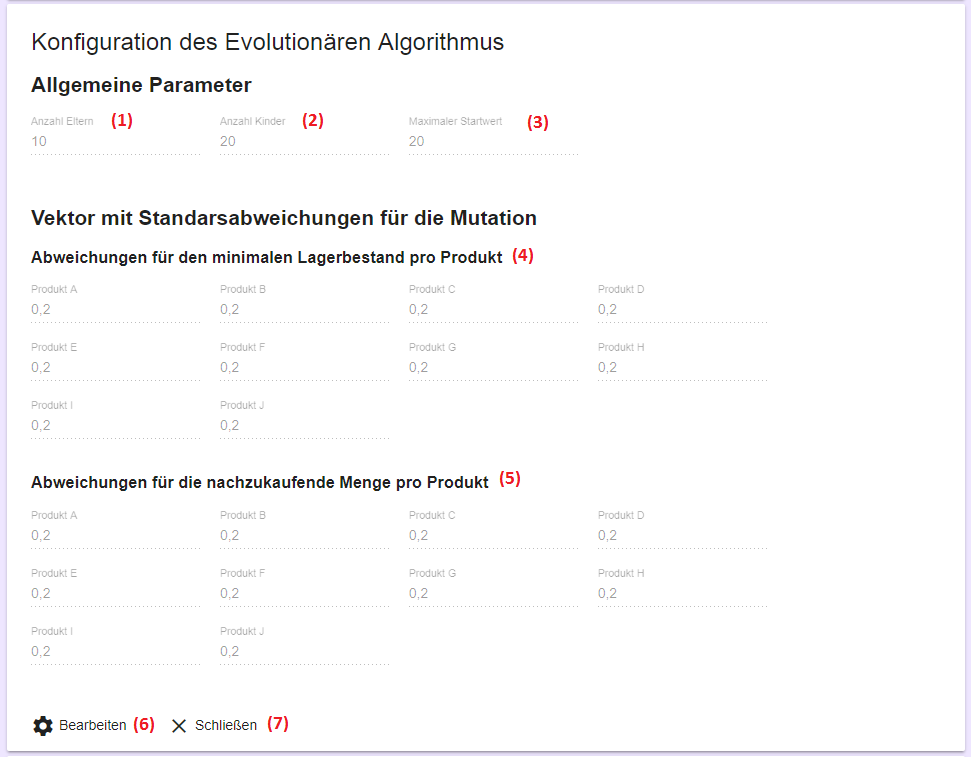
\includegraphics[width=0.8\textwidth]{res/config.png}
	\caption{Konfigurationsmöglichkeiten der ES}
	\label{img:config}
\end{figure}

Der letzte Teil des Benutzerinterfaces ist die Konfiguration der ES, welche bei Bedarf angepasst werden kann und in Abbildung \ref{img:config} dargestellt ist. Die einstellbaren Parameter sind:

\begin{itemize}
	\item (1) Anzahl der Eltern
	\item (2) Anzahl der entstehenden Kinder
	\item (3) Der Maximale Wert eines Attributs des Vektors bei der initialen Generierung
	\item (4) Die Standardabweichung des minimalen Lagerbestands pro Produkt
	\item (5) Die Standardabweichung der nachzukaufenden Menge pro Produkt
\end{itemize}

Das Bearbeiten kann mittels (6) gestartet werden. Dieses Button wechselt dann auf Speichern, was die eingetragenen Konfigurationen in das System übernimmt und den Zustand mit den neuen Parametern zurücksetzt. Zuletzt kann die Konfiguration mit (7) abgebrochen werden.

\newpage
\section{Logik des unterliegenden Systems}
\label{logik}

Wie bereits erwähnt wird für diesen Anwendungsfall eine Evolutionsstrategie verwendet. Dazu wird zu Beginn zufällig ein Satz an Eltern-Vektoren generiert, welche dann von der ES weiterverwendet werden. Ohne weitere Konfigurationen handelt es sich um eine (10/2,20)- Evolutionsstrategie. Die Anzahl der Vektoren ist dabei aber anpassbar. Der Crossover und die Mutation der Kinder ist dabei Fix. Die Tatsache, dass Eltern nicht in eine neuen Generation übernommen werden können ist ebenfalls statisch und kann nicht verändert werden. Die weiteren Eingenschaften der ES werden nachfolgend genauer dargestellt.

\subsection{Codierung der Vektoren}
\label{codierung}
Bei der Codierung der Vektoren handelt es sich um eine reelle Codierung. Sie bildet direkt die beiden Attribute \textit{minimaler Lagerbestand} und \textit{nachzukaufende Menge} mit ihren konkreten Werten pro Produkt ab. Der minimale Lagerbestand sagt dabei aus, ab welcher Menge eine Bestellung aufgegeben wird. Diese Bestellung beinhaltet dann die Menge, welche innerhalb des zweiten Parameters hinterlegt ist. Die Implementierung ist statisch auf 10 Produkte festgelegt, daher werden im folgenden auch immer 10 Produkte betrachtet.

\subsection{Crossover}
\label{crossover}
Das Crossover basiert hier auf der Reellen Codierung und geschieht durch Mittelwertbildung. Dabei werden zwei zufällige Eltern-Vektoren ausgewählt und mittels folgender Funktion miteinander verheiratet:

\begin{lstlisting}[backgroundcolor=\color{lightgray}]
childMinStock.push(
	Math.round((parent1.minimalStock[index] +
		parent2.minimalStock[index]) / 2));
		
childBuyAmount.push(
	Math.round((parent1.buyAmount[index] +
		parent2.buyAmount[index]) / 2));
\end{lstlisting}

Dies stellt die Mittelwertbildung zwischen den beiden Eltern dar und wird entsprechend pro Produkt wiederholt. Im Anschluss an das Crossover erfolgt die Mutation der Kinder.

\subsection{Mutation}
\label{mutation}
Die Mutation eines Vektors basiert auf dem in der Vorlesung verwendeten Prinzip unter Verwendung eines Vektors mit Standardabweichungen. Hier steht pro Eintrag innerhalb des Vektors eine Standardabweichung zur Verfügung. Der Mutationswert wird dann entsprechend aus dem Wert der Codierung und der für diesen Eintrag hinterlegten Standardabweichung gebildet. Im Anschluss wird dieser zufällig auf den Ausgangswert des Vektors Addiert oder Subtrahiert. In der Konfiguration kann eine Standardabweichung für jeden Eintrag innerhalb des Vektors festgelegt werden. Ohne weitere Konfiguration ist dieser Wert für jeden Eintrag zu Beginn 0,2. Angemerkt werden sollte hier noch, dass der Vektor der Standardabweichungen selbst keiner Mutation oder Entwicklung unterworfen ist, sondern über den gesamten Verlauf statisch bleibt.

\subsection{Bewertungsfunktion}
\label{bewertung}
Bei der Bewertungsfunktion wurde sich in der finalen Version für nachfolgende Variante entschieden. Für jedes Produkt werden zwei Kriterien betrachtet.\\

Das erste Kriterium errechnet sich wie folgt:

\begin{center}
	\(|v(minimaler Bestand) - taeglicher Verbrauch * Lieferzeit | * Produktgroeße\)
\end{center}

Diese Kriterium beschreibt den minimalen Lagerbestand zu einem Produkt. Betrachtet wird konkret, wie viel Einheiten des Produktes vorhanden sind, wenn der Minimale Bestand des Vektors erreicht wurde und wie viele Einheiten bis zur Lieferung noch verbraucht werden. Gewichtet wird dieser Bestand dann noch mit der Produktgröße, um eine Gewichtung zwischen den Produkten vorzunehmen. Positive Abweichungen (Überfluss) und negative Abweichungen (Mangel) werden hier gleich behandelt.\\

Das zweite Kriterium errechnet sich wie folgt:

\begin{center}
	\(|v(Einkaufsmenge) - taeglicher Verbrauch * Lieferzeit | * Produktgroeße\)
\end{center}

Diese Kriterium beschreibt den Bestand eines Produktes nach Lieferung. Hier wird von der Einkaufsmenge des Vektors der Verbrauch durch die Lieferzeit abgezogen. Der entstehende Lagerbestand wird erneut mit der Produktgröße multipliziert. Auch hier werden Überschuss und Mangel gleich behandelt.\\

Diese Kriterien werden miteinander addiert und dann über alle Produkte hinweg aufsummiert. Die dadurch entstehende Summe wird als Bewertung oder Fitness für den entsprechenden Vektor verwendet. Die besten Vektoren sind bei dieser Bewertung die Vektoren mit der \textbf{geringsten Fitness}, da hier am wenigsten Mangel oder Überschuss erwartet wird.

\newpage
\section{Aufbau der Applikation}
\label{aufbau}
Das Framework zur Implementierung ist Angular. Es nimmt keine bedeutenden Eingriffe in die Implementierung der Logik, sondern übernimmt hauptsächlich die Darstellung innerhalb des Browsers.


Die Implementierung erfolgt innerhalb nachfolgender Orderstruktur:
\begin{lstlisting}[backgroundcolor=\color{lightgray}]
src
|- app
   |- ea
\end{lstlisting}
Außenstehende Komponenten sind zur Navigation und Verwaltung notwendig.

Innerhalb des EA-Ordners befinden sich folgende Dateien:
\begin{itemize}
\item ea.component.css (Styling der Komponente)
\item ea.component.html (Strukturierung der Komponente)
\item ea.component.ts (Logik der Komponente)
\end{itemize}

Im util-Ordner stehen noch weitere Klassen zur Verfügung, auf welche im Folgenden genauer eingegangen werden soll.
\begin{itemize}
	\item product.model.ts (Modell eines Produktes)
	\item vektoren.model.ts (Abbilden und Bewerten eines Vektors)
\end{itemize}

Die \textit{Produkt}-Klasse enthält alle für die Produkte notwendigen Informationen. Dies beinhaltet den Namen, die anteilige Lagergröße, die Lieferdauer, der Verbrauch und der Lagerbestand. Die Produkte an sich benötigen keine weitere Logik.\\

Die \textit{Vektoren}-Klasse besitzt zwei Arrays, welche für die reelle Codierung relevant sind: \textit{minimalStock} und \textit{buyAmount}. Innerhalb von minimalStock wird für jedes Produkt festgehalten, ab wann nachgekauft werden sollte, buyAmount enthält entsprechend die nachzukaufende Menge. Diese werden auch innerhalb der \textit{toString}-Methode zur Visualisierung verwendet. Hier werden sie allerdings jeweils Pro Produkt dargestellt, also [minimalStock(Prod A), buyAmount(Prod A)], ... (siehe Abbildung \ref{img:vektoren}). Ergänzt wird diese Darstellung durch die Bewertung der einzelnen Vektoren und eine durchschnittliche Fitness über die gesamte Generation.

Weiterhin stehen zwei Bewertungsfunktionen \textit{evaluate} und \textit{evaluate2} zur Verfügung. Es existieren zwei Funktionen, weil die erste Bewertungsfunktion keine zufriedenstellenden Ergebnisse lieferte, der Vollständigkeit halber aber weiterhin im Code hinterlegt ist. Genaueres dazu wird im Kapitel \ref{ergebnisse} erläutert. Für die Applikation wird aktuell nur die Methode \textit{evaluate2} verwendet, welche die Bewertung aus Kapitel \ref{bewertung} implementiert. Die weiteren Funktionen sind nur für die \textit{evaluate}-Methode relevant und werden daher hier nicht weiter erläutert.

Zuletzt bleibt noch die \textit{ea.component.ts}-Klasse. Aufgrund zeitlicher Engpässe übernimmt diese Klasse zwei Funktionalitäten und trennt diese nicht ganz sauber voneinander. Der eine Teil ist die Interaktion mit dem Frontend und der zweite Teil ist die Ausführung der Schritte der ES. Zur Speicherung der Informationen stehen folgende Attribute zur Verfügung:
\begin{itemize}
	\item \textbf{data}: Product[ ] (Ein Array, welches alle 10 Produkte enthält)
	\item \textbf{parents}: Vector[ ] (Ein Array, welches alle Eltern-Vektoren enthält)
	\item \textbf{children}: Vector[ ] (Ein Array, welches alle Kinder-Vektoren enthält)
	\item \textbf{averageFitness}: number (Wert der durchschnittlichen Fitness der Eltern)
	\item \textbf{bestVector}: Vector (Der beste Vektor, welcher innerhalb der Laufzeit entdeckt wurde)
	\item \textbf{numParents}: number (Die Anzahl der Eltern-Vektoren)
	\item \textbf{numChildren}: number (Die Anzahl der Kinder-Vektoren)
	\item \textbf{maxStartSize}: number (Der Maximale Wert eines Attributs des Vektors bei der initialen Generierung)
	\item \textbf{standardDeviationMinimalStock}: number[ ] (Ein Array der Standardabweichungen für den Minimalen Bestand eines Produktes)
	\item \textbf{standardDeviationbuyAmount}: number[ ] (Ein Array der Standardabweichungen für die Kaufmenge eines Produktes)
	\item \textbf{simulationIterations}: number (Anzahl der Iterationen für die \textit{evaluate}-Methode, nicht mehr relevant)
	\item \textbf{configForm}: FormGroup; (Ein Formular zum Auswerten der Konfigurationen des UI)
	\item \textbf{showConfig}: boolean (Schalter, um das Konfigurationsmenü anzuzeigen)
	\item \textbf{editConfig}: boolean (Schalter, um die Konfiguration zu bearbeiten)
\end{itemize}

Für die Interaktion mit dem Frontend sind folgende Funktionen implementiert:

\begin{itemize}
	\item \textbf{makeChildren} (Funktion hinter dem Button zum Generieren der Kinder)
	\item \textbf{evaluateVectors} (Funktion hinter dem Button zum Bewerten der  Vektoren)
	\item \textbf{buildNextGen} (Funktion hinter dem Button zum Mutieren und Bilden der näch"-sten Generation)
	\item \textbf{iterate} (Funktion zum wiederholen der ersten drei Schritte, Anzahl der Wiederholungen als Übergabeparameter)
	\item \textbf{editConfiguration} (Funktion zum Bearbeiten der Konfiguration)
	\item \textbf{closeConfiguration} (Funktion zum Schließen der Konfiguration)
	\item \textbf{saveConfiguration} (Funktion zum Anwenden einer neuen Konfiguration)
	\item \textbf{reset} (Zurücksetzen der Vektoren und generieren des Ausgangszustandes)
\end{itemize}


Die Funktionen für die Umsetzung der ES sollen etwas detaillierter erläutert werden. Die \textit{generateStart}-Methode stellt den Ausgangszustand der Elternvektoren her. Dabei wird die Anzahl der Eltern durch die der Art der ES bzw. der Konfiguration bestimmt. Die zufällige Generierung der Startwerte der einzelnen Vektoren ist ebenfalls von der hinterlegten Konfiguration abhängig.

Die Methode \textit{getChild} wendet die in Kapitel \ref{crossover} dargestellte Crossover-Funktion zwischen zwei Eltern dar. Dabei wird das zurückgegebene Kind direkt mutiert.

Die \textit{getNchildren}-Methode ist eine iterative Anwendung der \textit{getChild}-Methode in Abhän"-gigkeit der gewünschten Anzahl an Kindern. Zurückgegeben wird dementsprechend eine bereits mutierte Kinder-Generation.

Die \textit{mutate}-Methode wendet die in Kapitel \ref{mutation} auf einen Vektor und gibt entsprechend eine mutierte Variante davon zurück. Diese Funktion wird innerhalb der \textit{getChild}-Methode verwendet.

Die \textit{selectForNextGen}-Methode betrachtet alle Kinder-Vektoren und wählt die Vektoren mit der geringsten Fitness aus, um sie in die nächste Generation zu übertragen und als neue Eltern zu Verwenden.

Zuletzt berechnet die \textit{getAverageFitness}-Methode die durchschnittliche Fitness der Eltern-Vektoren, um diesen Wert im UI anzuzeigen.

\newpage
\section{Ergebnisse}
\label{ergebnisse}

\subsection{Unpassende Bewertungsfunktion}
Wie in den vorherigen Kapiteln bereits erwähnt wurde zu Beginn mit einer anderen Bewertungsfunktion gerechnet. Diese basierte auf einem Simulationsschema. In ihr wurde eine übergebene Anzahl an Tagen für das Lagersystem simuliert. Dazu wurden die Attribute jedes Vektors verwendet, um entsprechende Bestellungen aufzugeben, diese Bestellungen wurden dann nach entsprechender Zeit geliefert. Wenn der Bestand wieder unter den jeweiligen Wert viel, wurde dieses Prozedere wiederholt. Nach allen Tagen wurden die Fälle von leeren lagern und der durchschnittliche Lagerbestand für einen Vektor ermittelt und als Fitness verwendet. Wie erwähnt war diese Bewertung abhängig von der Anzahl der simulierten Tage. Hier wurde mit einigen unterschiedlichen Varianten experimentiert um festzustellen, dass die Vektoren zu diesem Punkt mutieren. Wenn Beispielsweise 100 Tage simuliert wurden, traten nach einigen Generationen Vektoren auf, welche Beispielsweise eine Bestellmenge von 100 Einheiten hatten. Dadurch mussten diese Vektoren nur ein einziges mal während der Simulation bestellen und sind nie auf ein Leeres Lager gestoßen. Es ist unschwer zu erkennen, dass dieses Ergebnis nicht besonders effizient ist, allerdings war es den Kommenden Generationen nicht möglich, dieses scheinbar lokale Maxima zu verlassen. Daraufhin wurde eine neue Bewertungsfunktion, ohne Simulationsdauer entworfen, welche in den vorhergehenden Kapiteln erläutert wurde.


\subsection{Gewichtung der Produkte basierend auf deren Größe}
In der verwendeten Bewertungsfunktion (Kapitel \ref{bewertung}) ist die Größe der jeweiligen Produkte für beide Kriterien relevant. Dies lässt sich ebenfalls in den entstehenden Generationen entnehmen.

\begin{figure}[htbp]
	\centering
	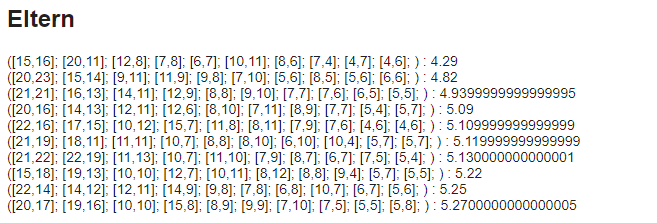
\includegraphics[width=0.9\textwidth]{res/gewicht_vektoren.png}
	\caption{Beispielergebnis mit der zweiten Bewertungsmethode}
	\label{img:vektoren_gewicht}
\end{figure}

Die Abbildung \ref{img:vektoren_gewicht} zeigt einen beliebigen, verhältnismäßig späten Zustand mit der zweiten Bewertungsfunktion. Zu erkennen it, dass die die Werte der ersten Produkte im Schnitt deutlich höher als die Werte der letzten Produkte sind. Dies lässt sich darauf zurückführen, dass die letzten Produkte den größten prozentualen Anteil innerhalb des Lagers in Anspruch nehmen und damit bei der Bewertung schwerer ins Gewicht fallen. Gesamtheitlich betrachtet ist diese Argumentation allerdings auch sinnvoll, da in der Tat dadurch Platz eingespart werden kann.\\

Hier sei noch eine kurze Anmerkung zu dieser Bewertungsfunktion gegeben. Die Funktion entscheidet wie erwähnt nicht, ob es sich um einen Überschuss oder einen Mangel an Produkten handelt. Eine sinnvolle Erweiterung dieser Bewertung wäre also Beispielweise eine höhere Gewichtung von Mangel. Das würde dazu führen, dass es wichtiger ist, dass ein Produkt überhaupt vorhanden ist, als nur wenige Tage nicht im Lager verfügbar ist.

\subsection{Die Anzahl der Kinder}
Zu Beginn der Simulation mutierten die Vektoren nicht zu sinnvollen Ergebnissen. Nach Überarbeitung der Bewertungsfunktion waren die Ergebnisse realistischer, jedoch konnten häufig keine nachvollziehbaren Maxima gefunden werden. Auch eine Anpassung der Standardabweichung hatte nicht die erhoffte Wirkung. Letztendlich wurde herausgefunden, dass eine Steigerung der Anzahl der Kinder zu dem erreichen der erhofften Maxima führte. Zu Beginn wurde mit einer (10/2,15)-ES gearbeitet. Als diese dann auf 20 oder sogar noch mehr Kinder erweitert wurden, konnte beobachtet werden, dass sich deutlich schneller, bessere Vektoren entwickeln. Das Verhältnis zwischen Erwachsenen und Kindern ist also ein wesentlicher Faktor bei dem Erfolg einer ES. 


\end{document}
